\documentclass[tikz]{standalone}
\usepackage{amsmath}
\usetikzlibrary{positioning,3d,calc,angles}

\begin{document}

\begin{tikzpicture}[x={(1cm,0cm)},y={(0cm,1cm)},z={(0.7cm,0.3cm)}]

\draw[fill=black, draw=none] (-1.5, -3) rectangle (7.5, 3);
\node (obs) at (0, 0) {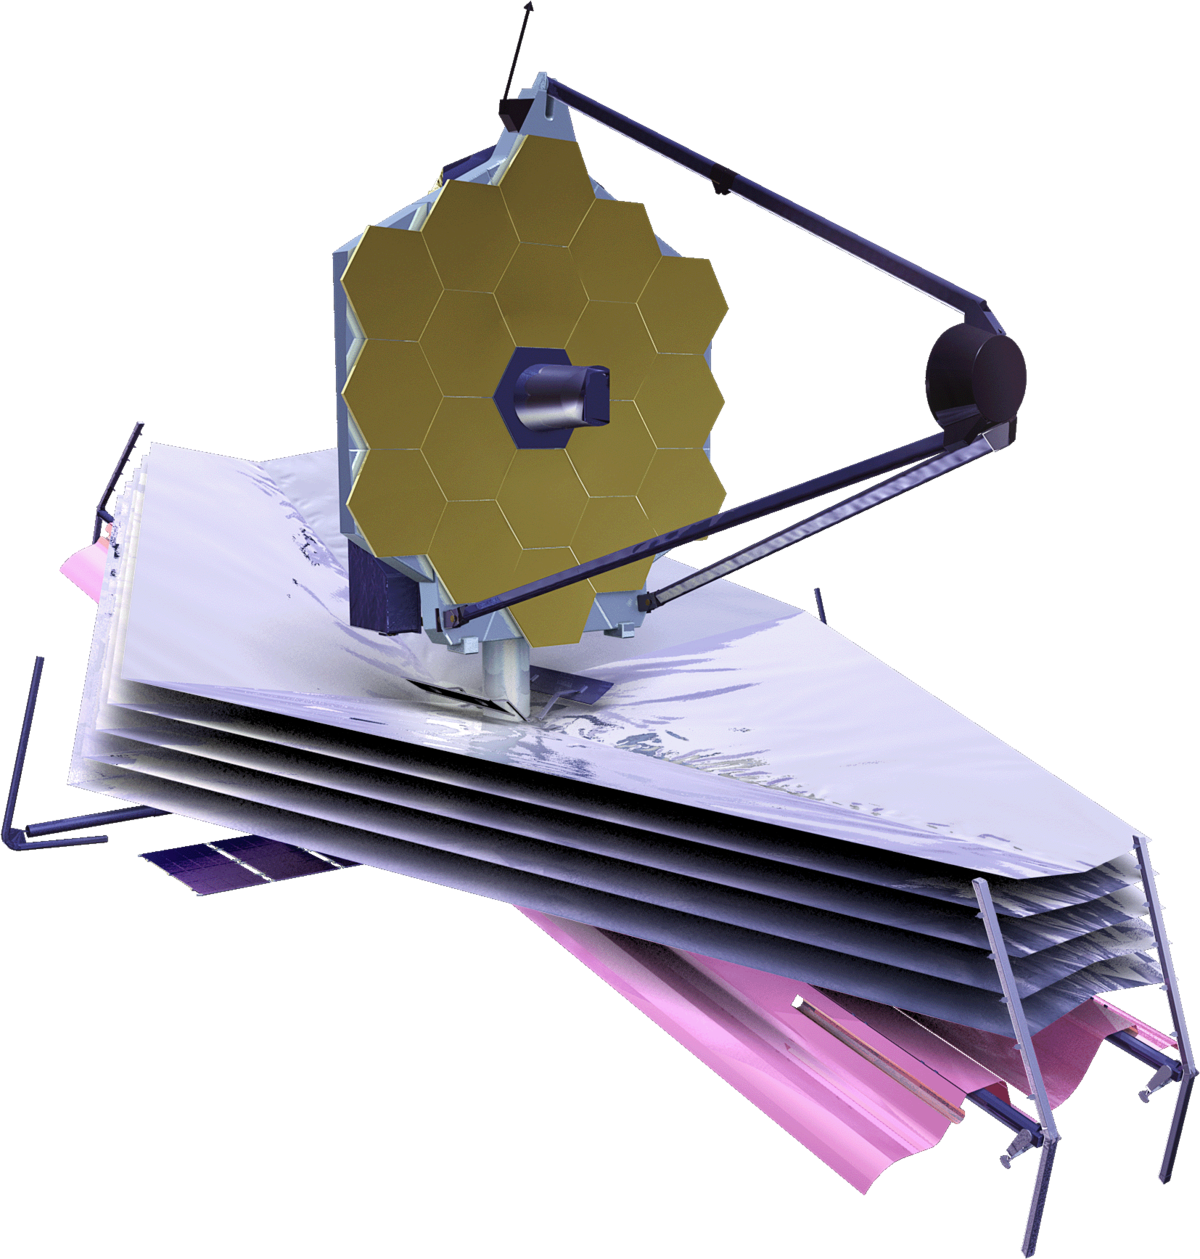
\includegraphics[width=2cm]{jwst_spacecraft}};

%\draw (3, -1, -1) -- ++(0, 3, 0) -- ++(0, 0, 3) -- ++(0, -3, 0) -- ++(0, 0, -3); 
%\draw (6, -1, -1) -- ++(0, 3, 0) -- ++(0, 0, 3) -- ++(0, -3, 0) -- ++(0, 0, -3); 


\draw[latex-latex, color=white] (0, -2.2) -- (6, -2.2) node[midway, below] {$D_{s}$};
\draw[latex-latex, color=white] (0, -2) -- (3, -2) node[midway, above] {$D_{\ell}$};
\draw[latex-latex, color=white] (3, -2) -- (6, -2) node[midway, above] {$D_{\ell s}$};



\coordinate (s) at (0.56, 0.41) ;
\coordinate (p) at (0., 0.38) ;
\coordinate (h) at (-0.1, 0.6) ;
\coordinate (s0) at (6, 0.8);
% m = 0.07, b=0.38
\coordinate (sl) at (3, 0.59);
\draw[latex-, color=white] (p) -- (s) -- (h) -- +(3, 1) coordinate (theta0);
\coordinate (xi0) at (3, 0.38);

\draw[dashed, color=white] (p) -- +(3, 0);

\draw[latex-, color=white] (1, 0.96) .. controls +(0.2, -0.3) and +(0, 0.1) .. (1.2, 0.38) node[midway, above right] {$\theta$};

\draw[dashed, color=white] (p) -- (sl);

\begin{scope}[canvas is zy plane at x=3, transform shape]
        \node (source) at (0, 0.5) {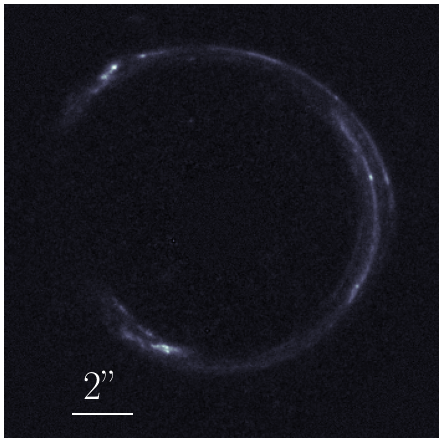
\includegraphics[height=3cm]{obs_horseshoe}};
        %\node[color=white] at (0, 2.2) {Plan de la lentille};
\end{scope}

\draw[dashed, color=white] (3, 0.38) -- +(3, 0);

\draw[color=white] (theta0) -- (s0); 

\draw[dashed , color=white] (theta0) -- +(3, 1) coordinate (sprime);

\draw[-latex, color=white] (4.1, 2.) .. controls +(0.2, -0.2) and +(0.1, 0.3) .. (4.2, 1.25) node[midway, right] {$\alpha$};

\draw[dashed, color=white] (sl) -- (s0);

\begin{scope}[canvas is zy plane at x=6, transform shape]
        \node (source) at (0, 0.5) {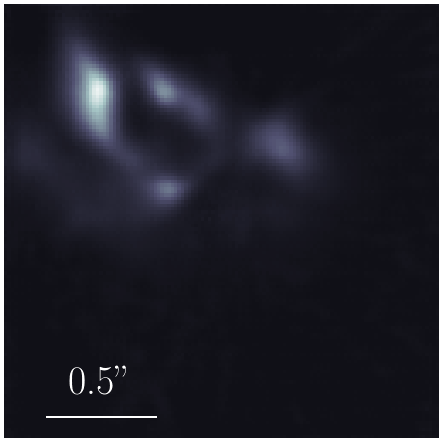
\includegraphics[height=3cm]{source_pred_horseshoe2}};
        %\node[color=white] at (0, 2.2) {Plan de la source};
\end{scope}


\draw[latex-, color=white] (4.2, 0.65) .. controls +(0.02, -0.1) and +(0, 0.1) .. (4.25, 0.38) node[midway, right] {$\beta$};

\draw[-latex, color=white] (6, 0.38) -- (s0) node[midway, right] {$\boldsymbol{ \eta} $};
\draw[-latex, color=white] (6, 0.38) -- (sprime) node[midway, right] {$\boldsymbol{ \eta}' $};

\draw[-latex, color=white] (3, 0.38) -- (theta0) node[midway, right] {$\boldsymbol{ \xi} $};
\draw[-latex, color=white] (3, 0.38) -- +(0.5, 0) node[midway, below] {$\mathbf{e}_{\parallel}$};
 
\end{tikzpicture}
\end{document}
